\newcommand{\PRnk}{\operatorname{Rank}}

\chapter{Random Walks}\label{ran_process_chap}

\term{Random Walks} are used to model situations in which an object
moves in a sequence of steps in randomly chosen directions.  For
example, physicists use three-dimensional random walks to model
Brownian motion and gas diffusion.  In this chapter we'll examine two
examples of random walks.  First, we'll model gambling as a simple
1-dimensional random walk---a walk along a straight line.  Then we'll
explain how the \idx{Google} search engine used random walks through
the graph of world-wide web links to determine the relative importance
of websites.

\section{Gambler's Ruin}

\begin{editingnotes}
In the Mathematical literature, random walks are for some reason
traditionally discussed in the context of some social vice.  A
one-dimensional random walk is often described as the path of a drunkard
who randomly staggers left or right at each step.  We'll examine
one-dimensional random walks using the language of gambling.
\end{editingnotes}

Suppose a gambler starts with an initial stake of $n$ dollars and
makes a sequence of \$1 bets.  If he wins an individual bet, he gets
his money back plus another \$1.  If he loses the bet, he loses the
\$1.

We can model this scenario as a random walk between integer points on
the real line.  The position on the line at any time corresponds to
the gambler's cash-on-hand, or \emph{capital}.  Walking one step to the
right corresponds to winning a \$1 bet and thereby increasing his
capital by \$1.  Similarly, walking one step to the left corresponds
to losing a \$1 bet.

The gambler plays until either he runs out of money or increases
his capital to a target amount of $T$ dollars.  The amount $T-n$ is
defined to be his \term{intended profit}.

If he reaches his target, he will have won his intended profit and is
called an overall \emph{winner}.  If his capital reaches zero before
reaching his target, he will have lost $n$ dollars; this is called
\term{going broke} or being \term{ruined}.  We'll assume that the
gambler has the same probability $p$ of winning each individual \$1
bet, and that the bets are mutually independent.  We'd like to find
the probability that the gambler wins.

The gambler's situation as he proceeds with his \$1 bets is illustrated in
Figure~\ref{LN12:fig:walk1}.  The random walk has boundaries at 0 and $T$.  If
the random walk ever reaches either of these boundary values, then it
terminates.

\begin{figure}
  \centerline{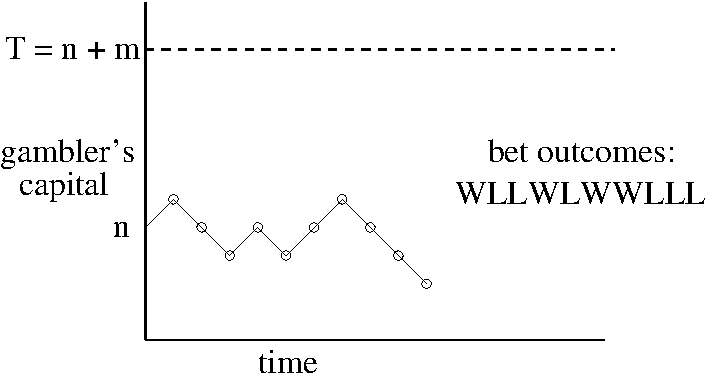
\includegraphics[height=2.5in]{walk1}}
  \caption{A graph of the gambler's capital versus time for one
    possible sequence of bet outcomes.  At each time step, the graph
    goes up with probability $p$ and down with probability $1-p$.  The
    gambler continues betting until the graph reaches either 0 or $T$.
    If he starts with \$$n$, his intended profit is \$$m$ where
    $T=n+m$.}
  \label{LN12:fig:walk1}
\end{figure}

In an \term{unbiased game}, the individual bets are fair: the gambler
is equally likely to win or lose each bet---that is, $p = 1/2$.  The
gambler is more likely to win if $p>1/2$ and less likely to win if
$p<1/2$; these random walks are called \term{biased}.  We want to
determine the probability that the walk terminates at boundary
$T$---the probability that the gambler wins.  We'll do this in
Section~\ref{prwinwalk_subsec}.  But before we derive the probability,
let's examine what it turns out to be.

\begin{editingnotes}

\textcolor{blue}{Make this a pset problem}

\subsection{The Probability Space}

Each random-walk game corresponds to a path like the one in
Figure~\ref{LN12:fig:walk1} that starts at the point $(n,0)$.  A winning path
never touches the $x$ axis and ends when it first touches the line $y=T$.
Likewise, a losing path never touches the line $y=T$ and ends when it first
touches the $x$ axis.

\textcolor{red}{figure causing errors omitted here}
\iffalse

\setlength{\unitlength}{0.0125in}
%
\begingroup\makeatletter\ifx\SetFigFont\undefined
% extract first six characters in \fmtname
\def\x#1#2#3#4#5#6#7\relax{\def\x{#1#2#3#4#5#6}}%
\expandafter\x\fmtname xxxxxx\relax \def\y{splain}%
\ifx\x\y   % LaTeX or SliTeX?
\gdef\SetFigFont#1#2#3{%
  \ifnum #1<17\tiny\else \ifnum #1<20\small\else
  \ifnum #1<24\normalsize\else \ifnum #1<29\large\else
  \ifnum #1<34\Large\else \ifnum #1<41\LARGE\else
     \huge\fi\fi\fi\fi\fi\fi
  \csname #3\endcsname}%
\else
\gdef\SetFigFont#1#2#3{\begingroup
  \count@#1\relax \ifnum 25<\count@\count@25\fi
  \def\x{\endgroup\@setsize\SetFigFont{#2pt}}%
  \expandafter\x
    \csname \romannumeral\the\count@ pt\expandafter\endcsname
    \csname @\romannumeral\the\count@ pt\endcsname
  \csname #3\endcsname}%
\fi
\fi\endgroup
\begin{picture}(300,175)(0,-10)
\path(40,160)(40,0)
\path(20,40)(300,40)
\dottedline{5}(20,140)(300,140)
\path(40,80)(60,100)(80,80)
	(100,100)(120,120)(140,100)
	(160,120)(180,100)(200,80)
	(220,60)(240,80)(260,100)
	(280,120)(300,140)
\put(0,140){\makebox(0,0)[lb]{\smash{{{\SetFigFont{12}{14.4}{rm}T}}}}}
\put(0,40){\makebox(0,0)[lb]{\smash{{{\SetFigFont{12}{14.4}{rm}0}}}}}
\put(60,20){\makebox(0,0)[lb]{\smash{{{\SetFigFont{12}{14.4}{rm}1}}}}}
\put(80,20){\makebox(0,0)[lb]{\smash{{{\SetFigFont{12}{14.4}{rm}2}}}}}
\put(100,20){\makebox(0,0)[lb]{\smash{{{\SetFigFont{12}{14.4}{rm}3}}}}}
\put(0,80){\makebox(0,0)[lb]{\smash{{{\SetFigFont{12}{14.4}{rm}n}}}}}
\end{picture}
\fi

Any length $k$ path can be characterized by the history of wins and
losses on individual \$1 bets, so we use a length $k$ string of $W$'s
and $L$'s to model a path, and assign probability $p^rq^{k-r}$ to a
string that contains $r$ occurrences of $W$.  The \emph{outcomes} in
our sample space will be precisely those string corresponding to
winning or losing walks, that is, when $r = 2k$.

What about the infinite walks in which the gambler plays forever, neither
reaching his target nor going bankrupt?  A recitation problem will show the
probability of playing forever is zero, so we don't need to include any
such outcomes in our sample space.

As a sanity check on this definition of the probability space, you
should verify that the sum of these outcome probabilities is one.

\iffalse
To do this, we let $X$ be any string of $W$'s and $L$'s, and let $[X]$ be
the event consisting of the outcomes that begin with $X$.  If $X$ itself
is not an outcome but begins with an outcome, then $[X] = \emptyset$ so
$\prob{[X]} = 0$.  On the other hand, if no prefix of $X$ is an outcome,
then it's easy to verify by induction on $k$ that $\prob{[X]} = p^rq^{k-r}$.
length $k$
\fi

\end{editingnotes}

%\subsection{The Probability of Winning}

%\subsubsection{The Unbiased Game}

Let's begin by supposing the gambler plays an unbiased game starting
with \$$100$ and will play until he goes broke or reaches a target of
$200$ dollars.  Since he starts equidistant from his target and
bankruptcy in this case, it's clear by symmetry that his probability
of winning is 1/2.

We'll show below that starting with $n$ dollars and aiming for a
target of $T \geq n$ dollars, the probability the gambler reaches his
target before going broke is $n/T$.  For example, suppose he wants to
win the same \$100, but instead starts out with \$500.  Now his
chances are pretty good: the probability of his making the 100 dollars
is $5/6$.  And if he started with one million dollars still aiming to
win \$100 dollars he almost certain to win: the probability is $1M/(1M
+ 100) > .9999$.

So in the unbiased game, the larger the initial stake relative to the
target, the higher the probability the gambler will win, which makes
some intuitive sense.  But note that although the gambler now wins
nearly all the time, when he loses, he loses \emph{big}. Bankruptcy
costs him \$1M, while when he wins, he wins only \$100.  The gambler's
average win remains zero dollars, which is what you'd expect when
making fair bets.

Another useful way to describe this scenario is as a game between two
players.  Say Albert starts with \$500, and Eric starts with \$100.
They flip a fair coin, and every time a Head appears, Albert wins \$1
from Eric, and vice versa for Tails.  They play this game until one
person goes bankrupt.  This problem is identical to the Gambler's Ruin
problem with $n=500$ and $T=100+500=600$.  The probability of Albert
winning is $500/600 = 5/6$.\iffalse , namely, the ratio of his wealth
to the combined wealth.  Eric's chance of winning is $1/6$.\fi

%\subsubsection{The Biased Game}

Now suppose instead that the gambler chooses to play roulette in an
American casino, always betting \$1 on red.  Because the casino puts
two green numbers on its roulette wheels, the probability of winning a
single bet is \iffalse 18/38, which is just\fi a little less than 1/2.
The casino has an advantage, but the bets are close to fair, and you
might expect that starting with \$500, the gambler has a reasonable
chance of winning \$100---the 5/6 probability of winning in the
unbiased game surely gets reduced, but perhaps not too drastically.

This mistaken intuition is how casinos stay in business.  In fact, the
gambler's odds of winning \$100 by making \$1 bets against the
``slightly'' unfair roulette wheel are less than 1 in 37,000.  If that's
surprising to you, it only gets weirder from here: 1 in 37,000 is in
fact an upper bound on the gambler's chance of winning
\emph{regardless of his starting stake}.  Whether he starts with
\$5000 or \$5 billion, he still has almost no chance of winning!

\subsection{The Probability of Avoiding Ruin}\label{prwinwalk_subsec}

We will determine the probability that the gambler wins using an idea
of Pascal's dating back to the beginnings probability theory in the
mid-seventeenth century.

Pascal viewed the walk as a two-player game between Albert and Eric as
described above.  Albert starts with a stack of $n$ chips and Eric
starts with a stack of $m = T-n$ chips.  At each bet, Albert wins
Eric's top chip with probability $p$ and loses his top chip to Eric
with probability $q \eqdef 1-p$.  They play this game until one
person goes bankrupt.

Pascal's ingenious idea was to alter the worth of the chips to make
the game fair regardless of $p$.  Specifically, Pascal assigned
Albert's bottom chip a worth of $r \eqdef q/p$ and then assigned
successive chips \emph{up} his stack worths equal to
$r^{2},r^{3},\dots$ up to his top chip with worth $r^n$.  Eric's top
chip gets assigned worth $r^{n+1}$, and the successive chips
\emph{down} his stack are worth $r^{n+2},r^{n+3},\dots$ down to
his bottom chip worth $r^{n+m}$.

The expected payoff of Albert's first bet is worth
\[
r^{n+1}\cdot p - r^n\cdot q
   = \paren{r^n \cdot \frac{q}{p}} \cdot p - r^n\cdot q = 0.
\]
so this assignment makes the first bet a fair one in terms of worth.
Moreover, whether Albert wins or loses the bet, the successive chip
worths counting up Albert's stack and then down Eric's remain
$r,r^2,\dots,r^n,\dots,r^{n+m}$, ensuring by the same reasoning that
every bet has fair worth.  So, Albert's expected worth at the end of
the game is the sum of the expectations of the worth of each bet,
which is 0.\footnote{Here we're legitimately appealing to infinite
  linearity, since the payoff amounts remain bounded independent of
  the number of bets.}

When Albert wins all of Eric's chips his total gain is worth
\[
\sum_{i=n+1}^{n+m} r^i,
\]
and when he loses all his chips to Eric, his total loss is worth
$\sum_{i=1}^n r^i$.  Letting $w_n$ be Albert's probability of winning,
we now have
\[
0 = \expect{\text{worth of Albert's payoff}} =
 w_n \sum_{i=n+1}^{n+m} r^i - (1-w_n)\sum_{i=1}^n r^i.
\]
In the truly fair game when $r=1$, we have $0 = mw_n - n(1-w_n)$, so
$w_n = n/(n+m)$, as claimed above.

In the biased game with $r\neq 1$, we have
\[
0 =   r \cdot \frac{r^{n+m} - r^{n}}{r-1} \cdot w_n
        - r \cdot \frac{r^{n}-1}{r-1}\cdot (1-w_n).
\]
Solving for $w_n$ gives
\begin{equation}\label{LN12:wnsol}
w_n = \frac{r^n-1}{r^{n+m} -1} = \frac{r^n-1}{r^{T} -1}
\end{equation}

We have now proved
\begin{theorem}\label{thm:gamblerruin}
  In the Gambler's Ruin game with initial capital $n$, target $T$,
  and probability $p$ of winning each individual bet,
\begin{equation}\label{eq:gamblerruin}
\prob{\text{the gambler wins}} =
\begin{cases}
 \dfrac{n}{T} & \text{ for } p = \dfrac{1}{2},\\
              &   \\
 \dfrac{r^n-1}{r^{T} -1} & \text{ for } p \neq \dfrac{1}{2},
\end{cases}
\end{equation}
where $r \eqdef q/p$.
\end{theorem}

\subsection{A Recurrence for the Probability of Winning}

Fortunately, you don't need to be as ingenuious Pascal in order to
handle Gambler's Ruin, because linear recurrences offer a methodical
approach to the basic problems.

The probability that the gambler wins is a function of his initial
capital $n$ his target $T \geq n$ and the probability $p$ that
the wins an individual one dollar bet.  For fixed $p$ and $T$, let
$w_n$ be the gambler's probability of winning when his initial
capital is $n$ dollars.  For example, $w_0$ is the probability that
the gambler will win given that he starts off broke and $w_T$ is the
probability he will win if he starts off with his target amount, so
clearly
\begin{align}
w_0 & = 0,\label{LN12:w0}\\
w_T & = 1. \label{LN12:wT}
\end{align}

Otherwise, the gambler starts with $n$ dollars, where $0 < n < T$.
Now suppose the gambler wins his first bet.  In this case, he is left
with $n+1$ dollars and becomes a winner with probability $w_{n+1}$.
On the other hand, if he loses the first bet, he is left with $n-1$
dollars and becomes a winner with probability $w_{n-1}$.  By the Total
Probability Rule, he wins with probability $w_n = p w_{n+1} + q
w_{n-1}$.  Solving for $w_{n+1}$ we have
\begin{equation}\label{LN12:rec1}
w_{n+1} = \frac{w_n}{p} - r w_{n-1}
\end{equation}
where $r$ is $q/p$ as in Section~\ref{prwinwalk_subsec}.

This recurrence holds only for $n+1 \leq T$, but there's no harm in
using~\eqref{LN12:rec1} to define $w_{n+1}$ for all $n+1 >1$.  Now, letting
\[
W(x) \eqdef w_0 + w_1x + w_2x^2 + \cdots
\]
be the generating function for the $w_n$, we derive from~\eqref{LN12:rec1}
and~\eqref{LN12:w0} using our generating function methods that
\iffalse
\[
W(x) -\frac{xW(x)}{p} + rx^2W(x) = w_1x,
\]
so
\fi
\begin{equation}\label{LN12:Wx}
W(x) = \frac{w_1x}{rx^2- x/p + 1}.
\end{equation}
But it's easy to check that the denominator factors:
\[
rx^2 - \frac{x}{p} + 1 = (1-x)(1-rx).
\]
Now if $p \neq q$, then using partial fractions we conclude that
\begin{equation}\label{LN12:WAB}
W(x) = \frac{A}{1-x} + \frac{B}{1-rx},
\end{equation}
for some constants $A,B$.  To solve for $A,B$, note that
by~\eqref{LN12:Wx} and~\eqref{LN12:WAB},
\[
w_1 x = A(1-rx) + B(1-x),
\]
so letting $x=1$, we get $A=w_1/(1-r)$, and letting $x=1/r$, we get
$B=w_1/(r-1)$.  Therefore,
\[
W(x) = \frac{w_1}{r-1} \paren{\frac{1}{1-rx} - \frac{1}{1-x}},
\]
which implies
\begin{equation}\label{LN12:withw1}
w_n = w_1\frac{r^n - 1}{r-1}.
\end{equation}
Finally, we can use~\eqref{LN12:withw1} to solve for $w_1$ by letting
$n=T$ to get \iffalse
\[
1=w_T = \frac{w_1}{r-1}\paren{r^T - 1}
\]
so
\fi
\[
w_1= \frac{r - 1}{r^T-1}.
\]
Plugging this value of $w_1$ into~\eqref{LN12:withw1}, we arrive at
the solution:
\[
w_n = \frac{r^n-1}{r^T -1},
\]
matching Pascal's result~\eqref{LN12:wnsol}.

In the unbiased case where $p=q$, we get from~\eqref{LN12:Wx} that
\[
W(x) = \frac{w_1 x}{(1-x)^2},
\]
and again can use partial fractions to match Pascal's
result~\eqref{eq:gamblerruin}.

\iffalse
Our derivation of~(\ref{LN12:wnsol}) ensures that it gives a formula for $w_n$
which satisfies~(\ref{LN12:rec1}) and has the right values at $n=0$ and $n=T$.
Moreover, the values determined by~(\ref{LN12:wnsol}) are the \emph{only ones}
that satisfy~\eqref{LN12:rec1} and the boundary conditions at $0$ and $T$,
though we won't prove this.  This implies that the Gambler's probability
of winning is indeed given by~\eqref{LN12:wnsol}.
\fi

\subsection{A simpler expression for the biased case}
The expression~\eqref{LN12:wnsol} for the probability that the Gambler
wins in the biased game is a little hard to interpret.  There is a
simpler upper bound which is nearly tight when the gambler's starting
capital is large and the game is biased \emph{against} the gambler.
Then $r >1$, both the numerator and denominator
in~\eqref{LN12:wnsol} are positive, and the numerator is smaller.
This implies that
\[
w_n < \frac{r^n}{r^T} = \paren{\frac{1}{r}}^{T-n}
\]
and gives:
\begin{corollary}\label{LN12:biaswincor}
  In the Gambler's Ruin game with initial capital $n$, target $T$,
  and probability $p < 1/2$ of winning each individual bet,
\begin{equation}\label{LN12:biaswinsimp}
\prob{\text{the gambler wins}} <  \paren{\frac{1}{r}}^{T-n} %\paren{\frac{p}{1-p}}^{T-n}
\end{equation}
where $r \eqdef q/p > 1$.
\end{corollary}

So the gambler gains his intended profit before going broke with
probability at most $1/r$ raised to the intended profit power.
Notice that this upper bound does not depend on the gambler's starting
capital, but only on his intended profit.  This has the amazing
consequence we announced above: \emph{no matter how much money he
  starts with}, if he makes \$1 bets on red in roulette aiming to win
\$100, the probability that he wins is less than
\[
\paren{\frac{18/38}{20/38}}^{100} = \paren{\frac{9}{10}}^{100} < \frac{1}{37,648}.
\]

The bound~\eqref{LN12:biaswinsimp} decreases exponentially as the
intended profit increases.  So, for example, doubling his intended
profit will square his probability of winning.  In this case, the
probability that the gambler's stake goes up $200$ dollars before he
goes broke playing roulette is at most
\[
(9/10)^{200} = ((9/10)^{100})^2 < \paren{\frac{1}{37,648}}^2,
\]
which is about 1 in 1.4 billion.

\begin{editingnotes}

The odds of winning a little money are not so bad.
Applying the exact formula~\eqref{LN12:wnsol}, we find that the probability
of winning \$10 before losing \$10 is
\[
\frac{\paren{\frac{20/38}{18/38}}^{10} - 1}
              {\paren{\frac{20/38}{18/38}}^{20} - 1}
  = 0.2585\dots.
\]
This is somewhat worse than the 1 in 2 chance in the fair game, but not
dramatically so.

\end{editingnotes}

\subsubsection{Intuition}

Why is the gambler so unlikely to make money when the game is only
slightly biased against him?  To answer this intuitively, we can
identify two forces at work on the gambler's wallet.  First, the
gambler's capital has random upward and downward \emph{swings} from
runs of good and bad luck.  Second, the gambler's capital will have a
steady, downward \emph{drift}, because the negative bias means an
average loss of a few cents on each \$1 bet.  The situation is shown
in Figure~\ref{fig:19P3}.

\begin{editingnotes}

For example, in roulette the gambler wins a dollar with probability $9/19$
and loses a dollar with probability $10/19$.  Therefore, his average
return on each bet is $9/10 - 10/19 = - 1/19 \approx -0.053$ dollars.
That is, on each bet his capital is can be expected to drift downward by a
little over 5 cents.

\end{editingnotes}

Our intuition is that if the gambler starts with, say, a billion
dollars, then he is sure to play for a very long time, so at some
point there should be a lucky, upward swing that puts him \$100 ahead.
But his capital is steadily drifting downward.  If the gambler does
not have a lucky, upward swing early on, then he is doomed.  After his
capital drifts downward by tens and then hundreds of dollars, the size
of the upward swing the gambler needs to win grows larger and larger.
And as the size of the required swing grows, the odds that it occurs
decrease exponentially.  As a rule of thumb, \emph{drift dominates
  swings} in the long term.

\begin{figure}[h]

\graphic{gambler}

\caption{In a biased random walk, the downward drift usually dominates
  swings of good luck.}

\label{fig:19P3}

\end{figure}

\iffalse
\begin{figure}
\centerline{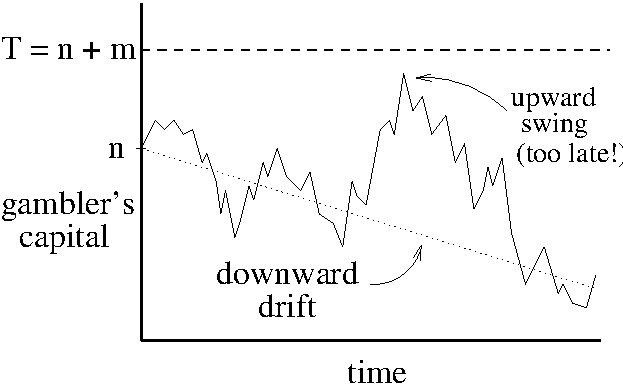
\includegraphics[height=2.5in]{walk2}}
\caption{\em In an unfair game, the gambler's capital swings randomly up
and down, but steadily drifts downward.  If the gambler does not have
a winning swing early on, then his capital drifts downward, and later
upward swings are insufficient to make him a winner.}
\label{LN12:fig:walk2}
\end{figure}
\fi

We can quantify these drifts and swings.  After $k$ rounds for $k \le
\min(m,n)$, the number of wins by our player has a binomial
distribution with parameters $p < 1/2$ and $k$.  His expected win on
any single bet is $p-q = 2p-1$ dollars, so his expected capital is
$n-k(1-2p)$.  Now to be a winner, his actual number of wins must
exceed the expected number by $m+k(1-2p)$.  But from the
formula~\eqref{eq:binom-var}, the binomial distribution has a standard
deviation of only $\sqrt{kp(1-p)}$ .  So for the gambler to win, he
needs his number of wins to deviate by
\[
\frac{m+k(1-2p)}{\sqrt{kp(1-2p)}}=\Theta(\sqrt{k})
\]
times its standard deviation.  In our study of binomial tails, we saw that
this was extremely unlikely.

In a fair game, there is no drift; swings are the only effect.  In the
absence of downward drift, our earlier intuition is correct.  If the
gambler starts with a trillion dollars then almost certainly there
will eventually be a lucky swing that puts him \$100 ahead.

\begin{editingnotes}
If we start with \$10 and play to win only \$10 more, then the difference
between the fair and unfair games is relatively small. We saw that the
probability of winning is $1/2$ versus about $1/4$.  Since swings of \$10
are relatively common, the game usually ends before the gambler's capital
can drift very far.  That is, the game does not last long enough for drift
to dominate the swings.
\end{editingnotes}


\subsection{How Long a Walk?}

Now that we know the probability $w_n$ that the gambler is a winner in
both fair and unfair games, we consider how many bets he needs on average
to either win or go broke.  A linear recurrence approach works here as well. 

\iffalse
\subsection{Duration of a Biased Walk}

Let $Q$ be the number of bets the gambler makes until the game ends.  

Since the gambler's expected win on any bet is $2p-1$, Wald's
Theorem should tell us that his game winnings $G$ will have
expectation $\expect{Q}(2p-1)$.  That is,
\begin{equation}\label{LN12:gw}
\expect{G} = (2p-1)\expect{Q},
\end{equation}

In an unbiased game~(\ref{LN12:gw}) is trivially true because both $2p-1$ and
the expected overall winnings $\expect{G}$ are zero.
On the other hand, in the unfair case $2p-1 \neq 0$.  Also, we know that
\[
\expect{G} = w_n(T-n) - (1-w_n)n = w_nT-n.
\]
So assuming~(\ref{LN12:gw}), we conclude
\begin{theorem}\label{LN12:ExQthm}
In the biased Gambler's Ruin game with initial capital $n$ target
$T$ and probability $p \neq 1/2$ of winning each bet,
\begin{equation}\label{LN12:ExQ}
\expect{\text{number of bets}} =
\frac{\prob{\text{the gambler wins}}T-n}{2p-1}.
\end{equation}
\end{theorem}

The only problem is that~\eqref{LN12:gw} is not a special case of Wald's
Theorem because $G = \sum_{i=1}^Q G_i$ is not a sum of \emph{nonnegative}
variables: when the gambler loses the $i$th bet, the random variable $G_i$
equals $-1$.  However, this is easily dealt with.\footnote{The random variable
$G_i+1$ is nonnegative, and $\expcond{G_i+1}{Q \geq i} =
\expcond{G_i}{Q\geq i}+1 = 2p$, so by Wald's Theorem
\begin{equation}\label{LN12:G1}
\expect{\sum_{i=1}^Q (G_i+1)}  = 2p\expect{Q}.
\end{equation}
But
\begin{eqnarray}
\expect{\sum_{i=1}^Q (G_i+1)} & = & \expect{\sum_{i=1}^Q G_i + \sum_{i=1}^Q 1}\notag\\
   & = & \expect{(\sum_{i=1}^Q G_i) + Q}\notag\\
   & = & \expect{\sum_{i=1}^Q G_i} + \expect{Q}\notag\\
   & = & \expect{G} + \expect{Q}\label{LN12:GQ}.
\end{eqnarray}
Now combining~(\ref{LN12:G1}) and~(\ref{LN12:GQ}) confirms the truth of our
assumption~(\ref{LN12:gw}).}

\begin{example}
If the gambler aims to profit \$100 playing roulette with $n$ dollars to
start, he can expect to make $((n+100)/37,648 - n)/(2(18/38) - 1) \approx
19n$ bets before the game ends.  So he can enjoy playing for a good while
before almost surely going broke.
\end{example}

\subsection{Duration of an Unbiased Walk}

This time, we need the more general approach of recurrences to handle the
unbiased case.  
\fi

For fixed $p$ and $T$, let $e_n$ be the expected number of bets until
the game ends when the gambler's initial capital is $n$ dollars.
Since the game is over in zero steps if $n=0$ or $T$, the boundary
conditions this time are $e_0=e_T=0$.

Otherwise, the gambler starts with $n$ dollars, where $0 < n < T$.
Now by the conditional expectation rule, the expected number of steps
can be broken down into the expected number of steps given the outcome
of the first bet weighted by the probability of that outcome.  But
after the gambler wins the first bet, his capital is $n+1$, so he can
expect to make another $e_{n+1}$ bets.
That is,
\[
\expcond{\#\text{bets starting with } \$n}{\text{gambler wins first bet}} = 1 + e_{n+1}.
\]
Similarly, after the gambler loses his first bet, he can expect to
make another $e_{n-1}$ bets:
\[
\expcond{\#\text{bets starting with } \$n}{\text{gambler loses first bet}} = 1 + e_{n-1}.
\]
So we have
\begin{align*}
e_n & = p\expcond{\#\text{bets starting with } \$n}{\text{gambler wins first bet}} +
      q\expcond{\#\text{bets starting with } \$n}{\text{gambler loses first bet}}\\
    & = p(1 + e_{n+1}) +  q(1 + e_{n-1}) =  pe_{n+1} + qe_{n-1} + 1.
\end{align*}
This yields the linear recurrence
\begin{equation}\label{expected-bets-recurrence}
e_{n+1} = \frac{1}{p} e_n - \frac{q}{p} e_{n-1} - \frac{1}{p}.
\end{equation}
\iffalse
For $p = q = 1/2$, this simplifies to
\begin{equation}\label{expected-fair-bets-recurrence}
e_{n+1} = 2e_n - e_{n-1} - 2.
\end{equation}

\fi

The routine solution of this linear recurrence yields:
\begin{theorem}\label{ExQthm}
In the Gambler's Ruin game with initial capital $n$, target
$T$, and probability $p$ of winning each bet,
\begin{equation}\label{expectedbets}
\expect{\text{number of bets}} =
 \begin{cases}
 n(T-n) & \text{ for } p = \dfrac{1}{2},\\
          \\ 
\dfrac{w_n  \cdot T - n}{p-q} %\frac{r^n - 1}{r^T - 1}%pr{\text{the gambler wins}}
       & \text{ for } p \neq \dfrac{1}{2}\\
       & \text{where } w_n = (r^n - 1)/(r^T - 1)\\
       & \qquad = \prob{\text{the gambler wins}}.
\end{cases}
\end{equation}
\end{theorem}

In the unbiased case,~\eqref{expectedbets} can be rephrased simply as
\begin{equation}\label{capital.profit}
\expect{\text{number of fair bets}} = \text{initial capital}
\cdot \text{intended profit}.
\end{equation}
For example, if the gambler starts with \$10 dollars and plays until
he is broke or ahead \$10, then $10 \cdot 10 = 100$ bets are required
on average.  If he starts with \$500 and plays until he is broke or
ahead \$100, then the expected number of bets until the game is over
is $500 \times 100 = 50,000$.  This simple
formula~\eqref{capital.profit} cries out for an intuitive proof, but
we have not found one (where are you, Pascal?).

\iffalse

\textcolor{blue}{Below is my try at the suggestion of Santosh and Adam
  Kalai for an example requiring a Pairwise \emph{Uncorrellated}
  Sampling Theorem.  But I don''t think this goes anywhere.}

\subsection{Fluctuations in an Unbiased Walk}

Let's consider the probability that the game ends within $k$ flips.  This
number is awkward to calculate explicitly, but we will be able to estimate
it using our methods for estimating expected deviation from the mean.

Let $C_k$ be the gamblers capital after $k$ flips.  That is,
\[
C_k \eqdef n + \sum_{i=1}^k G_i.
\]
In the unbiased case, the expected win on one flip is zero, so since $C_k$
is the sum of variables which have expectation 0, it follows that
$\expect{C_k} = 0$.  What about $\variance{C_k}$?  We will prove that
\begin{equation}\label{LN12:sumvarg}
\variance{C_k} = \sum_{i=1}^k \variance{G_i}.
\end{equation}

Note that for $i \neq j$, $G_i$ and $G_j$ are not independent, and so we
cannot appeal to pairwise independent additivity of variance to
prove~(\ref{LN12:sumvarg}).  For example, if $G_i = 0$, then the game has
stopped before the $i$th flip, so if $j > i$, then $G_j = 0$.  On the
other hand, the probability that $G_j = 0$ is less than one, because there
is some positive probability that the game will continue for more than $j$
flips (except for the degenerate case when $n=1 and T=2$).  That is,
\[
\prcond{G_j = 0}{G_i = 0} = 1 > \prob{G_j = 0},
\]
confirming nonindependence.

However, inspection of the proof of pairwise independent additivity of
variance shows that it didn't really require pairwise independence!  The
only property of the variables being added is that they be pairwise
\emph{uncorrelated}:

\begin{definition*}
Random variables $R$ and $S$ are \emph{uncorrelated} iff
\begin{equation}\label{LN12:uncor}
\expect{RS} = \expect{R}\expect{S}.
\end{equation}
\end{definition*}

\begin{lemma}\label{LN12:Guncor}
For $i \neq j$, $G_i$ and $G_j$ are uncorrelated.
\end{lemma}

\begin{proof}
By symmetry $\pr{G_iG_j = 1} = \pr{G_iG_j = -1}$, and so
$\expect{G_iG_j} = 0 = \expect{G_i}\expect{G_j}$
\end{proof}
\fi

\subsection{Quit While You Are Ahead}

\begin{editingnotes}
label section as optional.
\end{editingnotes}

Suppose that the gambler never quits while he is ahead.  That is, he
starts with $n>0$ dollars, ignores any target $T$, but plays until he
is flat broke.  Call this the \term{unbounded Gambler's ruin} game.
It turns out that if the game is not favorable, that is, $p \leq 1/2$,
the gambler is sure to go broke.  In particular, this holds in an
unbiased game with $p = 1/2$.

\begin{editingnotes}
If the unbounded game is favorable to the gambler, \ie $p>1/2$, then
there is a positive probability that the gambler will play forever,
see Problem~\TBA{insert problem}.
\end{editingnotes}

\begin{lemma}\label{LN12:go broke}
If the gambler starts with one or more dollars and plays a fair
unbounded game, then he will go broke with probability 1.
\end{lemma}

\begin{proof}
If the gambler has initial capital $n$ and goes broke in a game without
reaching a target $T$, then he would also go broke if he were playing and
ignored the target.  So the probability that he will lose if he keeps
playing without stopping at any target $T$ must be at least as large as the
probability that he loses when he has a target $T>n$.

But we know that in a fair game, the probability that he loses is $1 -
n/T$.  This number can be made arbitrarily close to 1 by choosing a
sufficiently large value of $T$.  Hence, the probability of his losing
while playing without any target has a lower bound arbitrarily close to 1,
which means it must in fact be 1.
\end{proof}

So even if the gambler starts with a million dollars and plays a
perfectly fair game, he will eventually lose it all with probability
1.  But there is good news: if the game is fair, he can ``expect'' to
play forever:

\begin{lemma}\label{LN12:play forever}
If the gambler starts with one or more dollars and plays a fair
unbounded game, then his expected number of plays is infinite.
\end{lemma}

\begin{editingnotes}
\begin{proof}
Let $u_n$ be the expected number of bets for the unbounded game
to end with initial capital $n>0$.  Also, choose any $T \geq n$, and as
above, let $e_n$ be the expected number of bets for the game to end
when the gambler's target is $T$.

The unbounded game will have a larger expected number of bets compared
to the game with target $T$ because, in addition to the possibility
that the gambler goes broke, in the game with target $T$ there is also
the possibility that the game will end when the gambler reaches his
target.  So by~\eqref{capital.profit},
\[
u_n \geq e_n = n(T-n).
\]
Since $T$ may be any number greater than or equal to $n>0$, this lower
bound on $u_n$ can be arbitrarily large, which implies that $u_n$ must
be infinite.
\end{proof}
\end{editingnotes}

A proof appears in Problem~\ref{CP_gambler_unfair_forever}.

So even starting with just one dollar, the expected number of plays
before going broke is infinite!  This sounds reassuring---you can go
about your business without worrying about being doomed, because doom
will be infinitely delayed.  To illustrate a situation where you
really needn't worry, think about mean time to failure with a really
tiny probability of failure in any given second---say $10^{-100}$.  In
this case you are unlikely to fail any time much sooner than many
lifetimes of the estimated age of the universe, even though you will
eventually fail with probability one.

But in general, you shouldn't feel reassured by an infinite expected
time to go broke.  For example, think about a variant Gambler's Ruin
game which works as follows: run one second of the process that has a
$10^{-100}$ of failing in any second.  If it does \emph{not} fail,
then you go broke immediately.  Otherwise, you play a fair, unbounded
Gambler's Ruin game.  Now there is an overwhelming probability,
namely, $1-10^{-100}$, that you will go broke immediately.  But there
is a $10^{-100}$ probability that you will wind up playing fair
Gambler's Ruin, so your overall expected time will be at least
$10^{-100}$ times the expectation of fair Gambler's Ruin, namely, it
will still be infinite.

For the actual fair, unbounded Gambler's Ruin gain starting with one
dollar, there is a a 50\% chance the Gambler will go broke after the
first bet, and a more than $15/16$ chance of going broke within five
bets, for example.  So infinite expected time is not much consolation
to a Gambler who goes broke quickly with high probability.

\begin{editingnotes}
verify the 15/16 claim.
\end{editingnotes}

\iffalse

But don't assume this means that the
gambler is \emph{likely} to play for long---there is even a 50\%
chance he will lose the very first bet and go broke right away.

In fact, if the game is unfavorable, then
Theorem~\ref{LN12:ExQthm} and Corollary~\ref{LN12:biaswincor} imply
that his expected time to go broke is essentially proportional to his
initial capital, that is, $\Theta(n)$.

Lemma~\ref{LN12:play forever} says that the gambler can ``expect'' to
play forever, while Lemma~\ref{LN12:go broke} says that he is certain
to go broke.

These facts sound contradictory, but they are sound
consequences of the technical mathematical definition of expectation.
The moral here, as in Section~\ref{infinite_expect_sec}, is that naive
intuition is unreliable when it comes to infinite expectation.

\fi

\begin{problems}
\practiceproblems
\pinput{TP_Biased_Gamblers_Ruin}

\classproblems
\pinput{CP_gambler_unfair_forever}
\pinput{CP_gambler_ruin_recurrences}
\pinput{CP_gambler_fair_expected_time}

\begin{editingnotes}
\homeworkproblems
DRAFT PS\_fair\_ruin\_probability

PS\_drunken\_sailor used in ran\_var\_chap
\end{editingnotes}

\end{problems}

\section{Random Walks on Graphs}\label{Google_sec}

\begin{editingnotes}

\hyperdef{page}{rank}{Random walks on graphs arise in all sorts of
  applications.  One interesting example is Google and page rank, which
  we'll explore in this section.}

\end{editingnotes}

The hyperlink structure of the World Wide Web can be described as a
digraph.  The vertices are the web pages with a directed edge from
vertex $x$ to vertex $y$ if $x$ has a link to $y$.  A digraph showing
part of the website for MIT subject 6.042, \emph{Mathematics for
  Computer Science}, is shown in Figure~\ref{6042_webgraph}.

\begin{figure}
\centerline{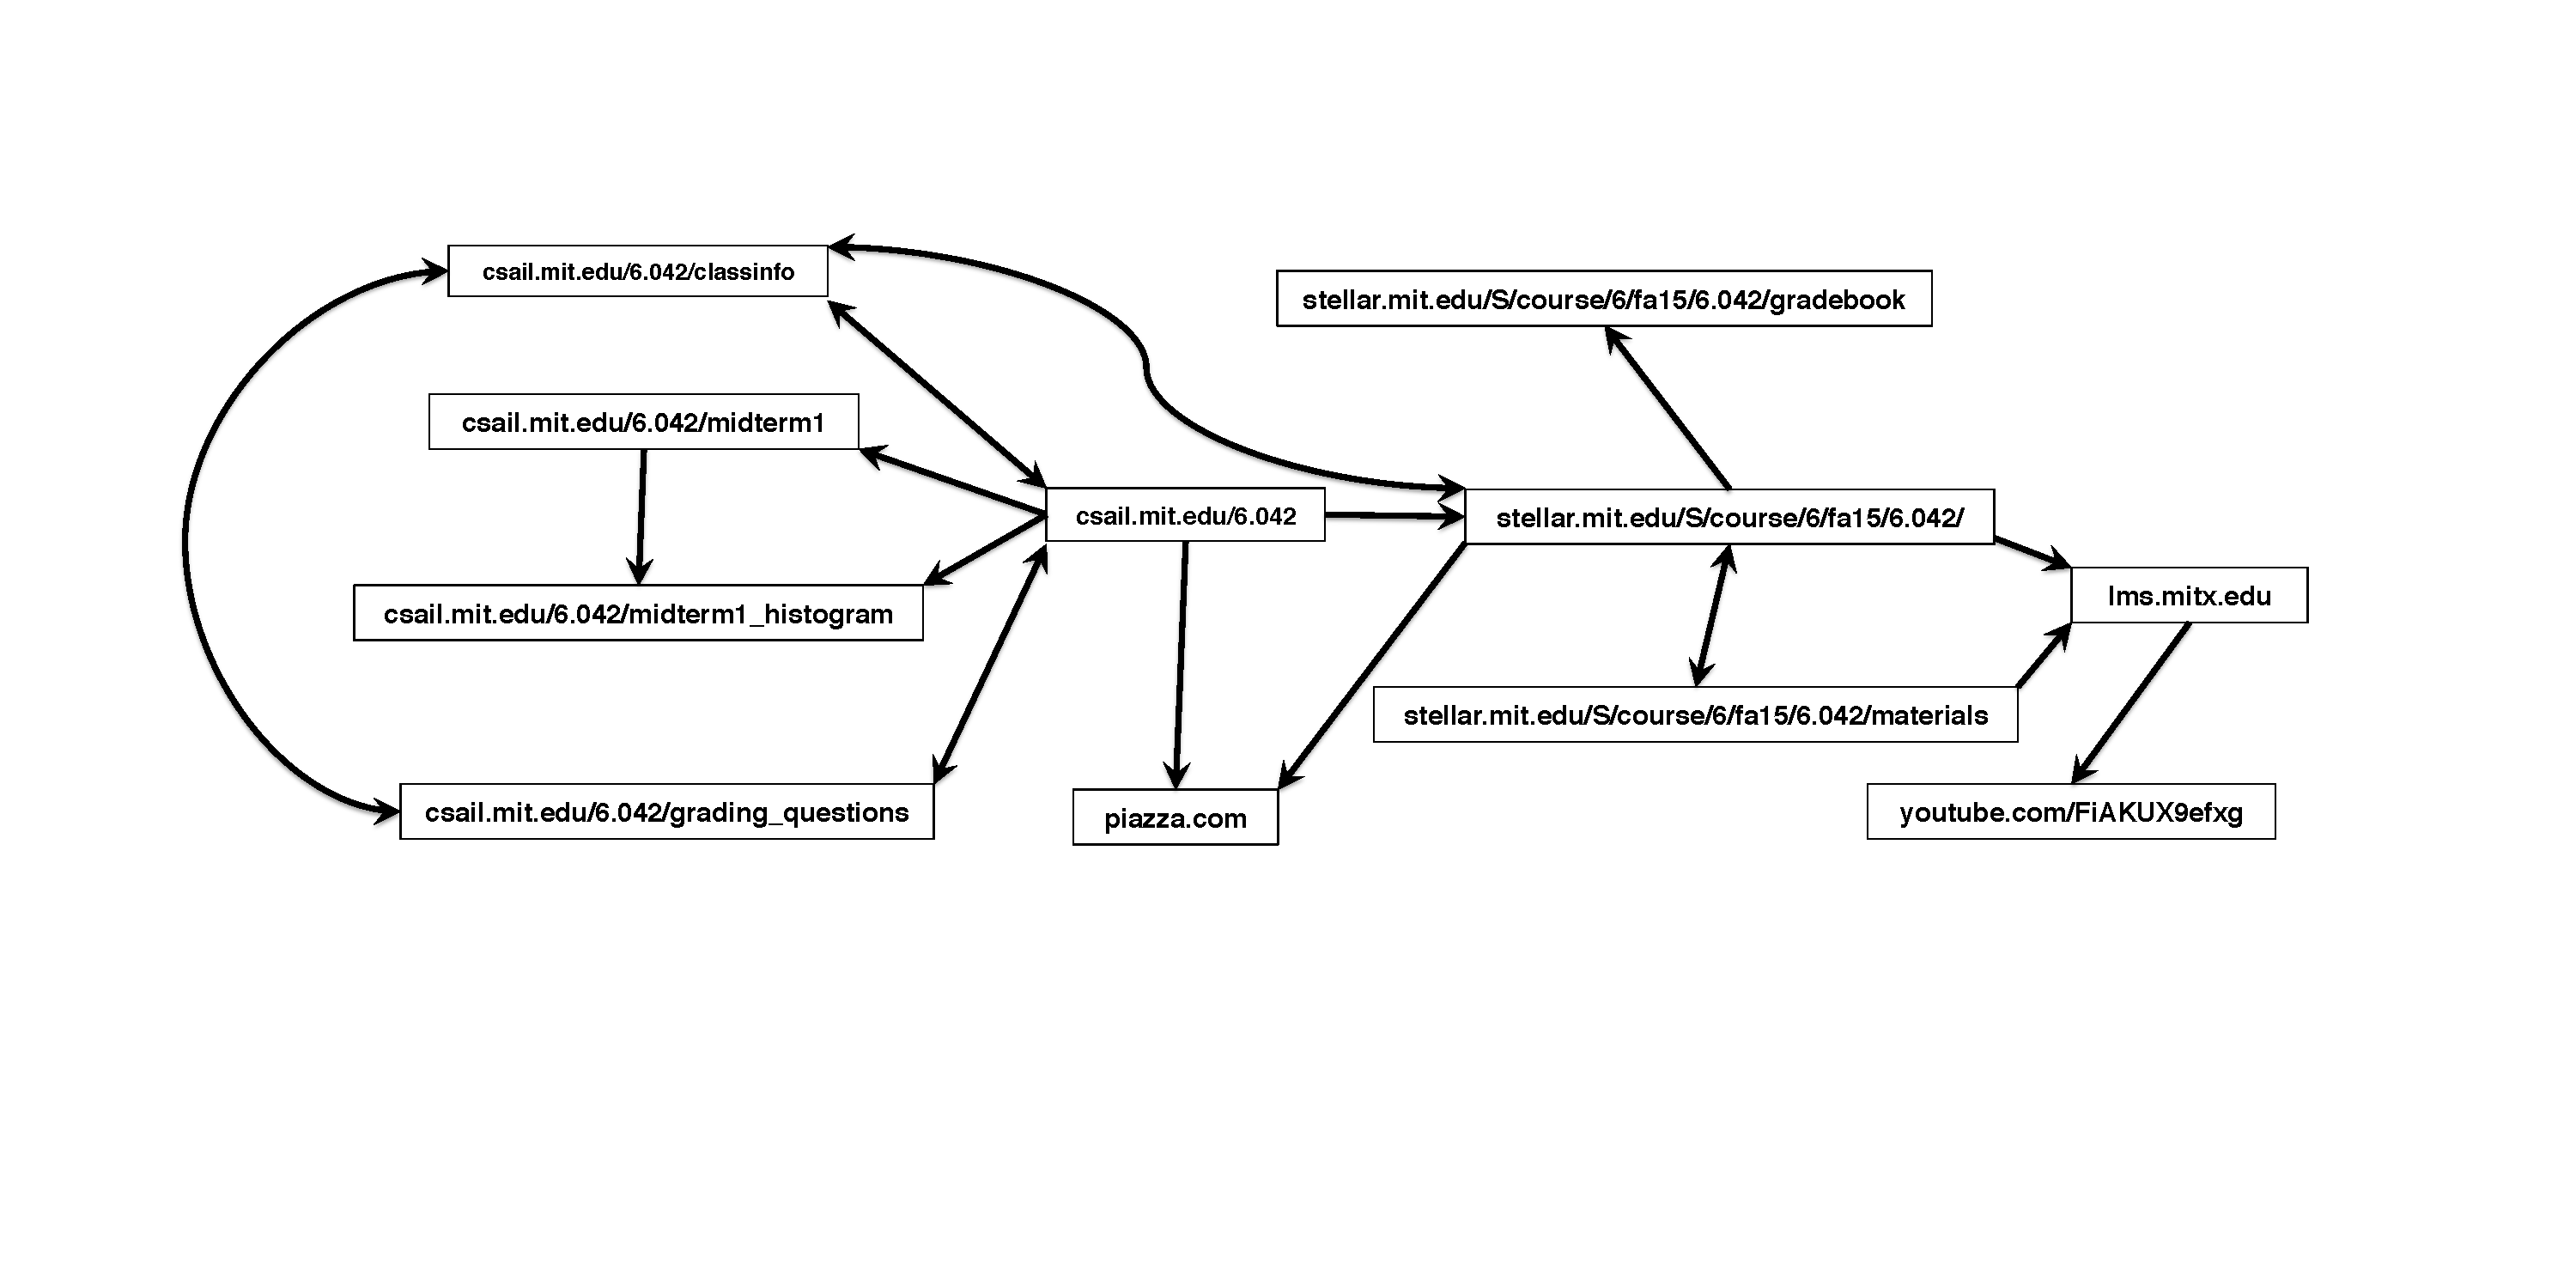
\includegraphics[height=3.5in]{website_digraph}}
\caption{Website digraph for MIT subject 6.042}
\label{6042_webgraph}
\end{figure}

The web graph is an enormous graph with trillions of vertices.
\iffalse
At first glance, this graph wouldn't seem to be very interesting.  But\fi
In 1995, two students at Stanford, \index{Page, Larry} Larry Page and
\index{Brin, Sergey} Sergey Brin, realized that the structure of this
graph could be very useful in building a search engine.  Traditional
document searching programs had been around for a long time and they
worked in a fairly straightforward way.  Basically, you would enter
some search terms and the searching program would return all documents
containing those terms.  A relevance score might also be returned for
each document based on the frequency or position that the search terms
appeared in the document.  For example, if the search term appeared in
the title or appeared $100$ times in a document, that document would
get a higher score.  \iffalse
So if an author wanted a document to get a higher
score for certain keywords, he would put the keywords in the title and
make it appear in lots of places.  You can even see this today with
some bogus web sites.\fi

This approach works fine if you only have a few documents that match a
search term.  But on the web, there are many billions of documents and
millions of matches to a typical search.  For example, on May 2, 2012,
a search on Google for `` `Mathematics for Computer Science' text''
gave 482,000 hits!  Which ones should we look at first?  Just because
a page gets a high keyword score---say because it has ``Mathematics
Mathematics $\dots$ Mathematics'' copied 200 times across the front of
the document---does not make it a great candidate for attention.  The
web is filled with bogus websites that repeat certain words over and
over in order to attract visitors.

\iffalse
One way to get placed high on the list is to pay Google an advertising
fee---and Google gets an enormous revenue stream from these fees.
Of course an early listing is worth a fee only if an advertiser's
target audience is attracted to the listing.  But an audience does get
attracted to Google listings because its ranking method is really good
at determining the most relevant web pages.\fi

Google's enormous market capital in part derives from the revenue it
receives from advertisers paying to appear at the top of search
results.  That top placement would not be worth much if Google's
results were as easy to manipulate as keyword frquencies.  Advertisers
pay because Google's ranking method is consistently good at
determining the most relevant web pages.  For example, Google
demonstrated its accuracy in our case by giving first
rank\footnote{First rank for some reason was an early version archived
  at Princeton; the Spring 2010 version on the MIT Open Courseware
  site ranked 4th and 5th.} to our 6.042 text.

So how did Google know to pick our text to be first out of
482,000?---because back in 1995 Larry and Sergey got the idea to allow
the digraph structure of the web to determine which pages are likely
to be the most important.

\subsection{A First Crack at Page Rank}

Looking at the web graph, do you have an idea which vertex/page might
be the best to rank first?  Assume that all the pages match the search
terms for now.  Well, intuitively, we should choose $x_2$, since lots
of other pages point to it.  This leads us to their first idea: try
defining the \term{page rank} of $x$ to be $\text{indegree}(x)$, the
number of links pointing to $x$.  The idea is to think of web pages as
voting for the most important page---the more votes, the better the rank.

Unfortunately, there are some problems with this idea.  Suppose you
wanted to have your page get a high ranking.  One thing you could do
is to create lots of dummy pages with links to your page.
\begin{center}
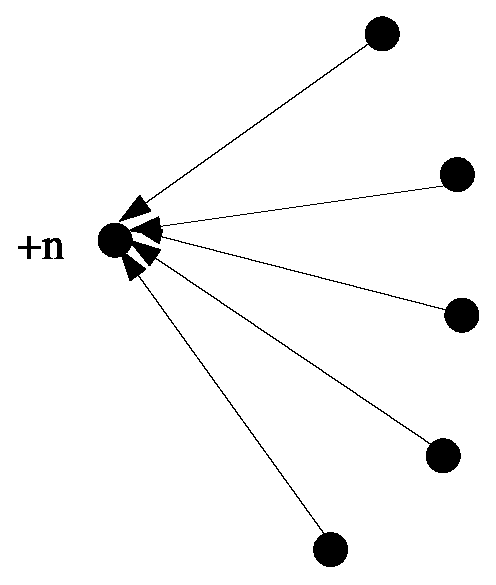
\includegraphics[width = 1.5in]{randomWalkFigs/dummy}
\end{center}

There is another problem---a page could become unfairly influential by
having lots of links to other pages it wanted to hype.
\begin{center}
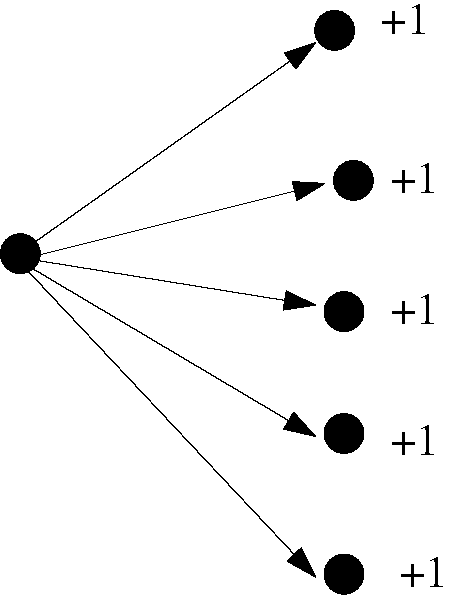
\includegraphics[width = 1.5in]{randomWalkFigs/outDegree}
\end{center}

So this strategy for high ranking would amount to, ``vote early, vote
often,'' which is no good if you want to build a search engine that's
worth paying fees for.  So, admittedly, their original idea was not so
great.  It was better than nothing, but certainly not worth billions of
dollars.

\subsection{Random Walk on the Web Graph}

But then Sergey and Larry thought some more and came up with a couple
of improvements.  Instead of just counting the indegree of a vertex,
they considered the probability of being at each page after a long
random walk on the web graph.  In particular, they decided to model a
user's web experience as following each link on a page with uniform
probability.  For example, if the user is at page $x$, and there are
three links from page $x$, then each link is followed with probability
$1/3$.  More generally, they assigned each edge $x \rightarrow y$ of
the web graph with a probability conditioned on being on page $x$:
\[
\prcond{\text{follow link}\ \diredge{x}{y}}{ \text{at page $x$}} \eqdef
\frac{1}{\outdegr{x}}.
\]
The simulated user experience is then just a \idx{random walk} on the
web graph.

We can also compute the probability of arriving at a particular page $y$
by summing over all edges pointing to $y$.  We thus have
\begin{eqnarray}
  \prob{\text{go to $y$}} &=&  \sum_{\text{edges}\ \diredge{x}{y}}
  \prcond{\text{follow link}\ \diredge{x}{y}}{\text{at page $x$}} \cdot
  \prob{\text{at page $x$}} \nonumber\\
  &=& \sum_{\text{edges}\ \diredge{x}{y}} \frac{\prob{\text{at
      $x$}}}{\outdegr{x}} \label{LN12:stepprob}
\end{eqnarray}
For example, in our web graph, we have
\[ \prob{\text{go to $x_4$}} = \frac{\prob{\text{at $x_7$}}}{2} +
\frac{\prob{\text{at $x_2$}}}{1} \ .
\]
One can think of this equation as $x_7$ sending half its probability
to $x_2$ and the other half to $x_4$.  The page $x_2$ sends all of its
probability to $x_4$.

There's one aspect of the web graph described thus far that doesn't
mesh with the user experience---some pages have no hyperlinks out.
Under the current model, the user cannot escape these pages.  In
reality, however, the user doesn't fall off the end of the web into a
void of nothingness.  Instead, he restarts his web journey.  Moreover,
even if a user does not get stuck at a dead end, they will commonly get
discouraged after following some unproductive path for a while and
will decide to restart.

To model this aspect of the web, Sergey and Larry added a
\emph{supervertex} to the web graph and added an edge from every page
to the supervertex.  Moreover, the supervertex points to every other
vertex in the graph with equal probability, allowing the walk to
restart from a random place.  This ensures that the graph is strongly
connected.

If a page had no hyperlinks, then its edge to the supervertex has to
be assigned probability one.  For pages that had some hyperlinks, the
additional edge pointing to the supervertex was assigned some
specially given probability.  In the original versions of Page Rank,
this probability was arbitrarily set to 0.15.  That is, each vertex
with outdegree $n \ge 1$ got an additional edge pointing to the
supervertex with assigned probability 0.15; its other $n$ outgoing
edges were still kept equally likely, that is, each of the $n$ edges
was assigned probability $0.85/n$.

\begin{editingnotes}
\TBA{Add figure}
\end{editingnotes}

\iffalse
For example, below left is a graph and below right is the same
graph after adding the supervertex $x_{N+1}$.

\bigskip\centerline{
  \resizebox{!}{1.3in}{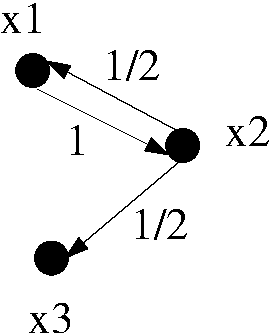
\includegraphics{randomWalkFigs/adjMatrix2}}
  \hspace{2cm}
  \resizebox{!}{1.5in}{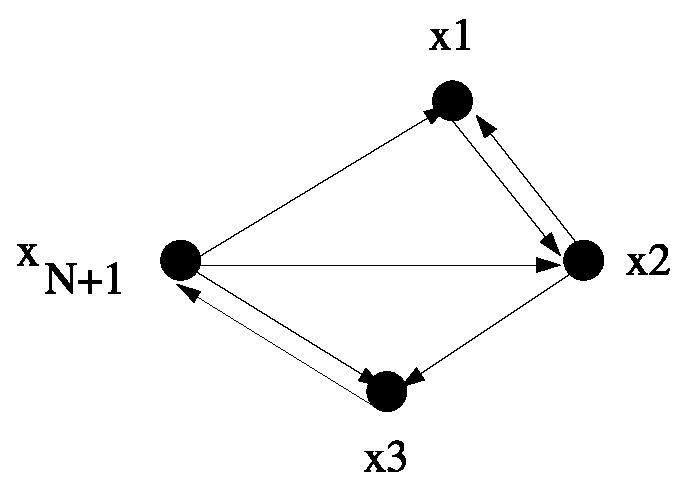
\includegraphics{randomWalkFigs/sinkGraph}}
}\bigskip

The addition of the supervertex also removes the possibility that the value
$1/\outdegr{x}$ might involve a division by zero.
\fi

\subsection{Stationary Distribution \& Page Rank}\label{stationary_sec}

The basic idea behind \idx{page rank} is finding a stationary
distribution over the web graph,
\begin{editingnotes}
(there are some more details, but this is the main idea)
\end{editingnotes}
so let's define a stationary distribution.

Suppose each vertex is assigned a probability that corresponds, intuitively,
to the likelihood that a random walker is at that vertex at a randomly
chosen time.  We assume that the walk never leaves the vertices in the graph,
so we require that
\begin{equation}\label{LN12:sum1}
\sum_{\text{vertices}\ x} \prob{\text{at $x$}} = 1.
\end{equation}

\begin{definition} An assignment of probabilities to vertices in a digraph
  is a \term{stationary distribution} if for all vertices $x$
\[
\prob{\text{at $x$}} = \prob{\text{go to $x$ at next step}}
\]
\end{definition}  

Sergey and Larry defined their page ranks to be a stationary distribution.
They did this by solving the following system of linear equations: find a
nonnegative number $\PRnk(x)$ for each vertex $x$ such that
\begin{equation}\label{LN12:PReqs}
\PRnk(x) = \sum_{\text{edges}\ \diredge{y}{x}} \frac{\PRnk(y)}{\outdegr{y}},
\end{equation}
corresponding to the intuitive equations given in \eqref{LN12:stepprob}.
These numbers must also satisfy the additional constraint corresponding
to~\eqref{LN12:sum1}:
\begin{equation}\label{LN12:sum1PR}
\sum_{\text{vertices}\ x} \PRnk(x) = 1.
\end{equation}

So if there are $n$ vertices, then equations~\eqref{LN12:PReqs}
and~\eqref{LN12:sum1PR} provide a system of $n+1$ linear equations in the
$n$ variables $\PRnk(x)$.  Note that constraint~\eqref{LN12:sum1PR}
is needed because the remaining constraints~\eqref{LN12:PReqs} could be
satisfied by letting $\PRnk(x)\eqdef 0$ for all $x$, which is useless.

Sergey and Larry were smart fellows, and they set up their page rank
algorithm so it would always have a meaningful solution.  Strongly
connected graphs have \emph{unique} stationary distributions
(Problem~\ref{PS_random_walk_strongly_connected}), and their addition
of a supervertex ensures this.  Moreover, starting from \emph{any}
vertex and taking a sufficiently long random walk on the graph, the
probability of being at each page will get closer and closer to the
stationary distribution.  Note that general digraphs without
supervertices may have neither of these properties: there may not be a
unique stationary distribution, and even when there is, there may be
starting points from which the probabilities of positions during a
random walk do not converge to the stationary distribution
(Problem~\ref{CP_random_walk_stationary_distributions_F13}).

\begin{editingnotes}
Here's a note on solving the system of linear constraints, for the
interested reader.

Let $W$ be the $n \times n$ with the entry $w_{ij}$ (in row $i$ and
column $j$) having the value $w_{ij} = 1/\text{outdegree}(x_i)$ if edge
$x_i \rightarrow x_j$ exists, and $w_{ij} = 0$ otherwise.  For example, in
our last example with the 4-vertex graph (including the supervertex), we have
$W$ given by:
\[
\left( \begin{array}{cccc}
    0 & 1 & 0 & 0 \\
    \frac{1}{2} & 0 & \frac{1}{2} & 0 \\
    0 & 0 & 0 & 1\\
    \frac{1}{3} & \frac{1}{3} & \frac{1}{3} & 0 \end{array} \right)
\]

The system of linear equations can now be described by a single matrix
vector product equation $W^T \vec{P} = \vec{P}$, where $W^T$ denotes the
transpose of $W$, and $\vec{P}$ is the column vector of page probabilities
(ranks):
\[\vec{P}\eqdef
\left( \begin{array}{c}
    \PRnk(x_1) \\
    \PRnk(x_2) \\
    \vdots \\
    \PRnk(x_n) \end{array} \right)
\]
So the $j$th entry of the solultion vector $\vec{P}$ is
\[
\sum_{1\leq i \leq n} w_{ij} \cdot \PRnk(x_i) =
\sum_{i \mid x_i \rightarrow x_j} \frac{\PRnk(x_i)}{\text{outdegree}(x_i)},
\]
which is exactly the constraint corresponding to vertex $x_j$
in~\eqref{LN12:PReqs}.

If you have taken a linear algebra or numerical analysis course, you
realize that the vector of page ranks is just the \emph{principle
  eigenvector} of the matrix $W$ of the web graph!  Once you've had such
a course, these values are easy to compute.  Of course, when you are
dealing with matrices of this size, the problem gets a little more
interesting.

\end{editingnotes}

Now just keeping track of the digraph whose vertices are trillions of
web pages is a daunting task.  That's why in 2011
\href{http://phys.org/news/2011-04-google-invests-million-solar-power.html}{Google
  invested \$168,000,000 in a solar power plant}---the electrical
power drawn by Google's servers in 2011 would have supplied the needs
of 200,000
households.\footnote{\href{http://www.nytimes.com/2011/09/09/technology/google-details-and-defends-its-use-of-electricity.html}
{\emph{Google Details, and Defends, Its Use of Electricity}, New York
  Times, September 8, 2011.}}  Indeed, Larry and Sergey named their
system Google after the number $10^{100}$---which is called a
``googol''---to reflect the fact that the web graph is so enormous.

Anyway, now you can see how this text ranked first out of 378,000
matches.  Lots of other universities used our notes and presumably
have links to the MIT Mathematics for Computer Science Open Course
Ware site, and the university sites themselves are legitimate, which
ultimately leads to the text getting a high page rank in the web
graph.

\begin{problems}
\practiceproblems
\pinput{TP_Random_Walks}
\pinput{TP_stable_distribution}
\pinput{TP_uncountable_stationary_distributions}

\classproblems
\pinput{CP_random_walk_stationary_distributions_F13}
\pinput{CP_stationary_distribution}
\pinput{CP_uniform_stationary}
\pinput{CP_simple_google_graph}

a\homeworkproblems
\pinput{PS_random_walk_strongly_connected}

\examproblems
\pinput{FP_uniform_stationary_distribution}
l
\end{problems}
\begin{editingnotes}
CONCLUSION?
\end{editingnotes}
\endinput
